% Chapter 5

\chapter{Conclusion \& Future Work} % Main chapter title

\label{Chapter5} % For referencing the chapter elsewhere, use \ref{Chapter1}

\lhead{Chapter 5. \emph{Conclusion \& Future Work}} % This is for the header on each page - perhaps a shortened title

%----------------------------------------------------------------------------------------

\begin{landscape}
\begin{figure}[h]
\centering
  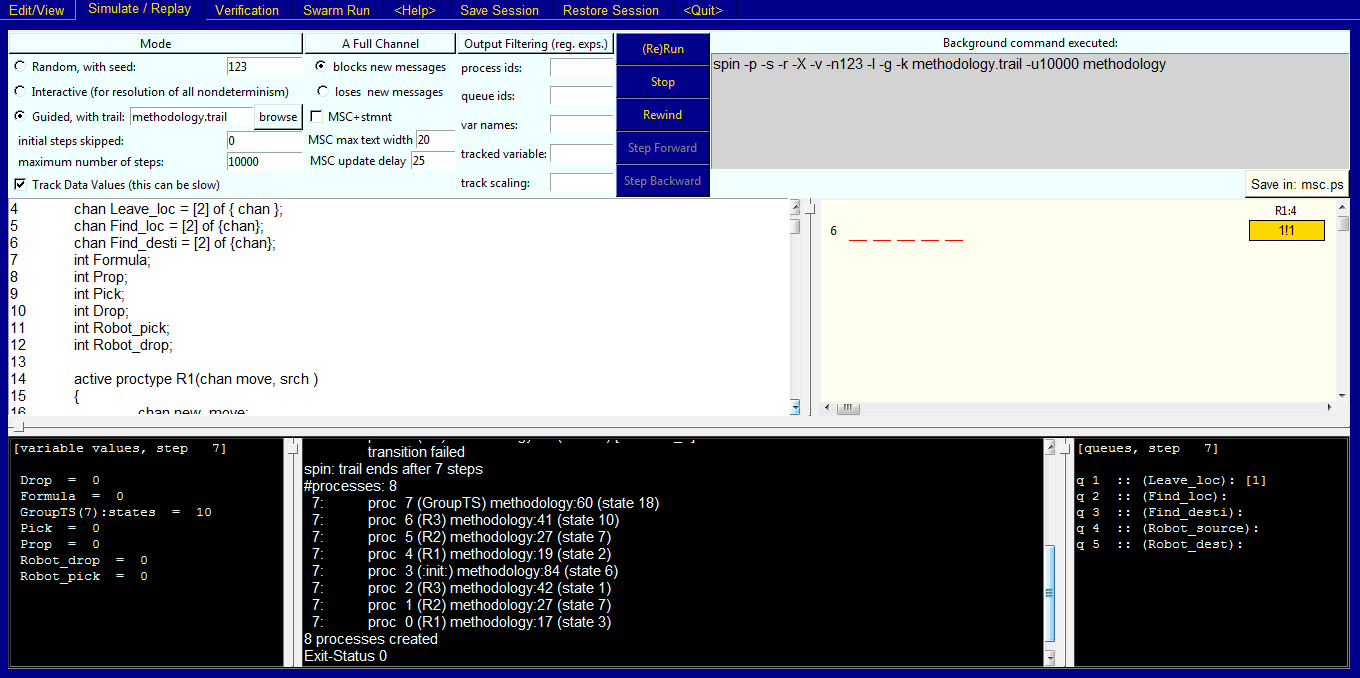
\includegraphics[width=19cm, height=13cm]{k}\\
  \caption{Result after simulation}
\end{figure}
\end{landscape}

\begin{landscape}
\begin{figure}[h]
\centering
  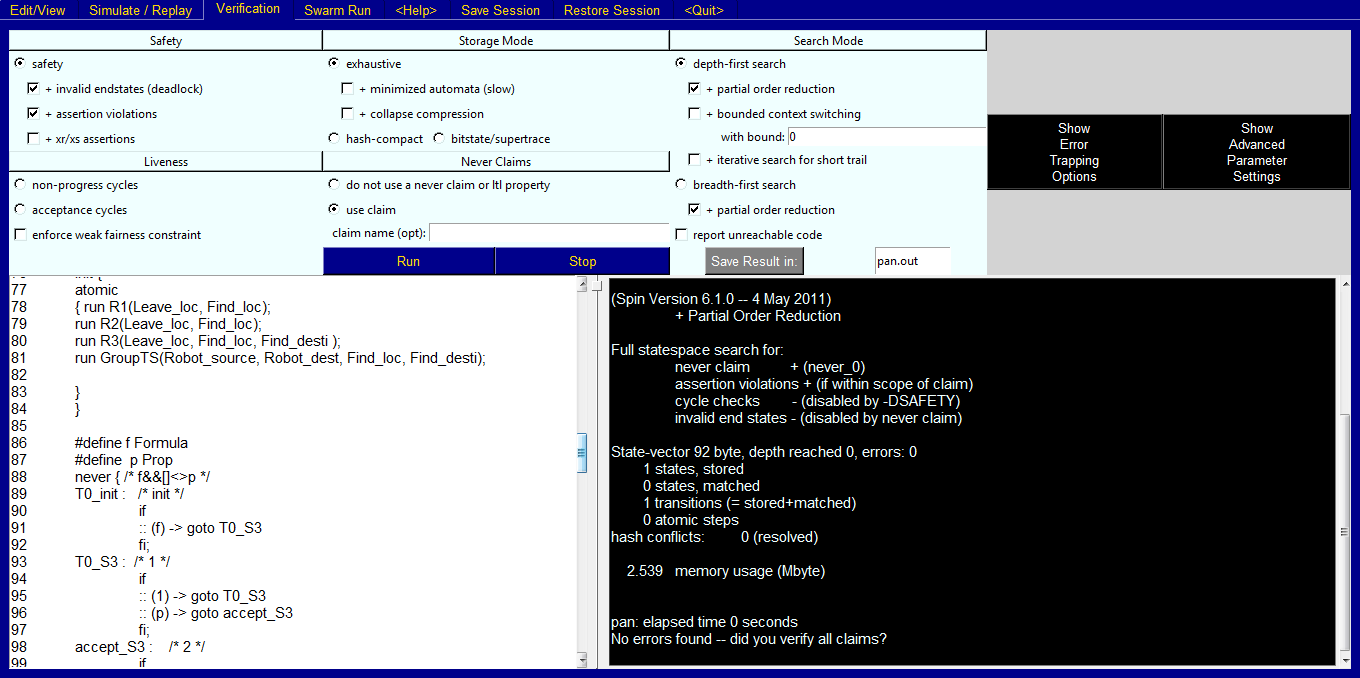
\includegraphics[width=19cm, height=13cm]{l}\\
  \caption{Result after verification}
\end{figure}
\end{landscape}

\pagebreak
\section{Conclusion}
A method is presented in this work for modeling the concurrent activities of a group of robots using temporal logics. The specifications are expressed in LTL formula and an algorithm is provided to model the transition system for the group of robots. Our method is optimal in a computational way as compared to previous methods, in which they constructed a model that captures all group members and their mission specification. The main drawback is the complexity of previous models that are time consuming processes.

Our approach is optimal to handle such cases where robots can take an action after confirmation of path availability according to the plan, and in some applications they has practical value where a series of different tasks performed by multiple robots in an environment. For some applications including new states and corresponding transitions to the structure of the robotic system may indicate to introducing advance stages or motion commands at some lower level. So the proper way in which the changes of these models are strictly application specific and we do not consider such details in our work. Assuming that these changes can be implemented in future.


